% Font options: 10pm, 11pt, 12pt
% Align headings left instead of center: nocenter
\documentclass[xcolor=x11names,compress]{beamer}\usepackage[]{graphicx}\usepackage[]{color}
%% maxwidth is the original width if it is less than linewidth
%% otherwise use linewidth (to make sure the graphics do not exceed the margin)
\makeatletter
\def\maxwidth{ %
  \ifdim\Gin@nat@width>\linewidth
    \linewidth
  \else
    \Gin@nat@width
  \fi
}
\makeatother

\definecolor{fgcolor}{rgb}{0.345, 0.345, 0.345}
\newcommand{\hlnum}[1]{\textcolor[rgb]{0.686,0.059,0.569}{#1}}%
\newcommand{\hlstr}[1]{\textcolor[rgb]{0.192,0.494,0.8}{#1}}%
\newcommand{\hlcom}[1]{\textcolor[rgb]{0.678,0.584,0.686}{\textit{#1}}}%
\newcommand{\hlopt}[1]{\textcolor[rgb]{0,0,0}{#1}}%
\newcommand{\hlstd}[1]{\textcolor[rgb]{0.345,0.345,0.345}{#1}}%
\newcommand{\hlkwa}[1]{\textcolor[rgb]{0.161,0.373,0.58}{\textbf{#1}}}%
\newcommand{\hlkwb}[1]{\textcolor[rgb]{0.69,0.353,0.396}{#1}}%
\newcommand{\hlkwc}[1]{\textcolor[rgb]{0.333,0.667,0.333}{#1}}%
\newcommand{\hlkwd}[1]{\textcolor[rgb]{0.737,0.353,0.396}{\textbf{#1}}}%
\let\hlipl\hlkwb

\usepackage{framed}
\makeatletter
\newenvironment{kframe}{%
 \def\at@end@of@kframe{}%
 \ifinner\ifhmode%
  \def\at@end@of@kframe{\end{minipage}}%
  \begin{minipage}{\columnwidth}%
 \fi\fi%
 \def\FrameCommand##1{\hskip\@totalleftmargin \hskip-\fboxsep
 \colorbox{shadecolor}{##1}\hskip-\fboxsep
     % There is no \\@totalrightmargin, so:
     \hskip-\linewidth \hskip-\@totalleftmargin \hskip\columnwidth}%
 \MakeFramed {\advance\hsize-\width
   \@totalleftmargin\z@ \linewidth\hsize
   \@setminipage}}%
 {\par\unskip\endMakeFramed%
 \at@end@of@kframe}
\makeatother

\definecolor{shadecolor}{rgb}{.97, .97, .97}
\definecolor{messagecolor}{rgb}{0, 0, 0}
\definecolor{warningcolor}{rgb}{1, 0, 1}
\definecolor{errorcolor}{rgb}{1, 0, 0}
\newenvironment{knitrout}{}{} % an empty environment to be redefined in TeX

\usepackage{alltt}
%\documentclass[xcolor=x11names,compress,handout]{beamer}
\usepackage[]{graphicx}
\usepackage[]{color}
\usepackage{booktabs}
\usepackage{hyperref}
\usepackage{tikz}
\usepackage{multirow}
\usepackage{dcolumn}
\usepackage{bigstrut}
\usepackage{amsmath} 
\usepackage{xcolor,colortbl}
\usepackage{amssymb}
%\newcommand{\done}{\cellcolor{teal}#1}

%% Beamer Layout %%%%%%%%%%%%%%%%%%%%%%%%%%%%%%%%%%
\useoutertheme[subsection=false,shadow]{miniframes}
\useinnertheme{default}
\usefonttheme{serif}
\usepackage{Arev}
\usepackage{pdfpages}

\setbeamerfont{title like}{shape=\scshape}
\setbeamerfont{frametitle}{shape=\scshape, size=\normalsize}

\definecolor{dkblue}{RGB}{0,0,102}

\setbeamercolor*{lower separation line head}{bg=dkblue} 
\setbeamercolor*{normal text}{fg=black,bg=white} 
\setbeamercolor*{alerted text}{fg=red} 
\setbeamercolor*{example text}{fg=black} 
\setbeamercolor*{structure}{fg=black} 
 
\setbeamercolor*{palette tertiary}{fg=black,bg=black!10} 
\setbeamercolor*{palette quaternary}{fg=black,bg=black!10} 

\renewcommand{\(}{\begin{columns}}
\renewcommand{\)}{\end{columns}}
\newcommand{\<}[1]{\begin{column}{#1}}
\renewcommand{\>}{\end{column}}

\setbeamertemplate{navigation symbols}{} 
\setbeamertemplate{footline}[frame number]
\setbeamertemplate{caption}{\raggedright\insertcaption\par}

\setbeamersize{text margin left=5pt,text margin right=5pt}

%%%%%%%%%%%%%%%%%%%%%%%%%%%%%%%%%%%%%%%%%%%%%%%%%%


\title{Making Causal Critiques}
\subtitle{Day 5 - Constructive Critiques}
\author{Jonathan Phillips}
\IfFileExists{upquote.sty}{\usepackage{upquote}}{}
\begin{document}

\frame{\titlepage}

\section{Constructive Critiques}

\begin{frame}
\frametitle{Being Constructive}
\begin{itemize}
\item Effective critiques are essential to learning
\begin{itemize}
\item We have a scholarly obligation to point out errors in reasoning
\item We learn collectively by collaborating
\item We learn individually by thinking critically about others' work
\end{itemize}
\item There is no research project that cannot be criticised
\end{itemize}
\end{frame}

\begin{frame}
\frametitle{Being Constructive}
\begin{itemize}
\item But criticism can also be used as a weapon
\begin{itemize}
\item To compete for attention/jobs
\item To discourage colleagues
\item To assert status/hierarchy/superiority
\item To destroy valuable research
\item To release our own frustrations
\end{itemize}
\end{itemize}
\end{frame}

\begin{frame}
\frametitle{Being Constructive}
\begin{itemize}
\item To avoid these risks, we must make our criticisms \textbf{constructive}
\begin{enumerate}
\item In terms of content
\item In terms of style
\end{enumerate}
\end{itemize}
\end{frame}

\section{Constructive Style}

\begin{frame}
\frametitle{Styles of Critique}
\begin{itemize}
\item Your task is to convince the author to \textit{improve} their work not to \textit{abandon} it
\item So they have to:
\begin{itemize}
\item Understand your comment
\item Not take it as a personal attack/become defensive
\item Have options for how to respond
\end{itemize}
\end{itemize}
\end{frame}

\begin{frame}
\frametitle{Styles of Critique}
\begin{itemize}
\item Always remember your comment might be wrong!
\begin{itemize}
\item You always know the data less well than the author
\item Recognize the inherent challenges and constraints of implementing the research
\end{itemize}
\item So phrase your comment in terms of 'as I understand your argument'
\item Or 'Could it be that something else is also happening?'
\end{itemize}
\end{frame}

\begin{frame}
\frametitle{Styles of Critique}
\begin{itemize}
\item Be specific! Which part of the research design is problematic?
\item Be concrete! Use an example/counterexample to communicate the risk
\item Be objective! We care about the research quality, not your personal opinion
\item Suggest an alternative
\end{itemize}
\end{frame}

\begin{frame}
\frametitle{Styles of Critique}
\begin{itemize}
\item Depersonalize criticism
\begin{itemize}
\item Instead of "you", refer to "in this type of research..."
\item "I feel like there might be some readers who..."
\end{itemize}
\item If in doubt, use the feedback sandwich:
\begin{itemize}
\item Something positive/encouraging
\item Critique
\item Something positive/encouraging
\end{itemize}
\end{itemize}
\end{frame}

\begin{frame}
\frametitle{Styles of Critique}
\begin{itemize}
\item Finally:
\begin{itemize}
\item Is the comment really necessary?
\item If it is a minor issue, is there a better way to communciate it?
\item If you have not fully understood, take time to invest in understanding it before commenting
\end{itemize}
\end{itemize}
\end{frame}

\section{Constructive Content}

\begin{frame}
\frametitle{Strengthening Causal Arguments}
\begin{enumerate}
\item Multiple tests
\item Multiple methods
\item Uncovering 'hidden' units
\item Heterogeneity tests
\item Placebo tests
\item Confirming Mechanisms
\end{enumerate}
\end{frame}

\begin{frame}
\frametitle{Multiple Tests}
\begin{itemize}
\item Learning requires the interaction of theory and evidence
\item Competing theories have multiple distinct implications
\item We should test \textit{all} of these implications
\end{itemize}
\end{frame}

\begin{frame}
\frametitle{Multiple Tests}
\begin{itemize}
\item For example, Deaton argues poor health causes low economic status, but observational data cannot rule out reverse causation. Additional tests to prove his claim include:
\begin{enumerate}
\item Whether the relationship falls after retirement
\item Whether the relationship is weaker among women, who on average work fewer hours
\item Whether the relationship holds even for diseases which could easily be cured with more income
\end{enumerate}
\end{itemize}
\end{frame}

\begin{frame}
\frametitle{Multiple Methods}
\begin{itemize}
\item Our methodologies' assumptions are often impossible to test in quantitative data
\item But qualitative evidence can help justify our assumptions
\item This means using multiple (mixed) methods
\begin{itemize}
\item Was randomization of a field experiment successful? We can interview people about the process
\item Are their spillovers (violations of SUTVA)? We can conduct a survey and find out where people got their information from
\item Can people migrate? We can use administrative data on migration rates to assess if these differences are large enough to explain our results
\item Is a regression discontinuity threshold enforced neutrally? Or was the threshold chosen to make sure a particular unit passed?
\item Is a geographic border discontinuity 'exogenous'? We can look in the archive to know how and why it was created
\end{itemize}
\item These are all "causal process observations" (Collier et al 2010)
\end{itemize}
\end{frame}

\begin{frame}
\frametitle{Multiple Methods}
\begin{itemize}
\item For example, Nunn (2008) asks whether the slave trade explains underdevelopment in parts of Africa, using an instrumental variable for distance to the Americas
\item Qualitative evidence helps:
\begin{itemize}
\item To verify that slaves usually sailed from the nearest port, and not a different country
\item To inform the need for extra controls, eg. for legal system, natural resources
\item To identify the direction of the selection bias - reverse causation is less of a problem because he shows the richest ethnic groups were most affected by the slave trade
\item To establish the exclusion restriction for the instrumental variable: that plantations were set up in the Carribean because of the climate, not because they were near the supply of slaves in West Africa
\end{itemize}
\end{itemize}
\end{frame}

\begin{frame}
\frametitle{Uncovering 'Hidden' Units}
\begin{itemize}
\item If our sample size is small and good comparisons are difficult to make, one strategy is to identify more units
\item Those units are often 'hidden', either because we did not think about them or there is no data on them
\item We can expand our dataset and adjust our research question
\item For example, John Londregan's talk 'uncovered' non-trading product-country pairs to provide another source of variation to explain
\end{itemize}
\end{frame}

\begin{frame}
\frametitle{Uncovering 'Hidden' Units}
\begin{itemize}
\item For example, Lewis (2016) wanted to ask whether ethnicity affected the formation of rebel groups, as many authors had argued
\item But there is a selection/survival bias in the data - we only have data on the groups that \textit{succeeded}
\item She collected data from Uganda on \textit{all} rebel groups
\begin{itemize}
\item Expanding the sample from 1 (in most datasets) to 15
\item Showing that ethnicity does not affect rebel group formation, but may affect their success
\end{itemize}
\end{itemize}
\end{frame}

\setbeamercolor{background canvas}{bg=}
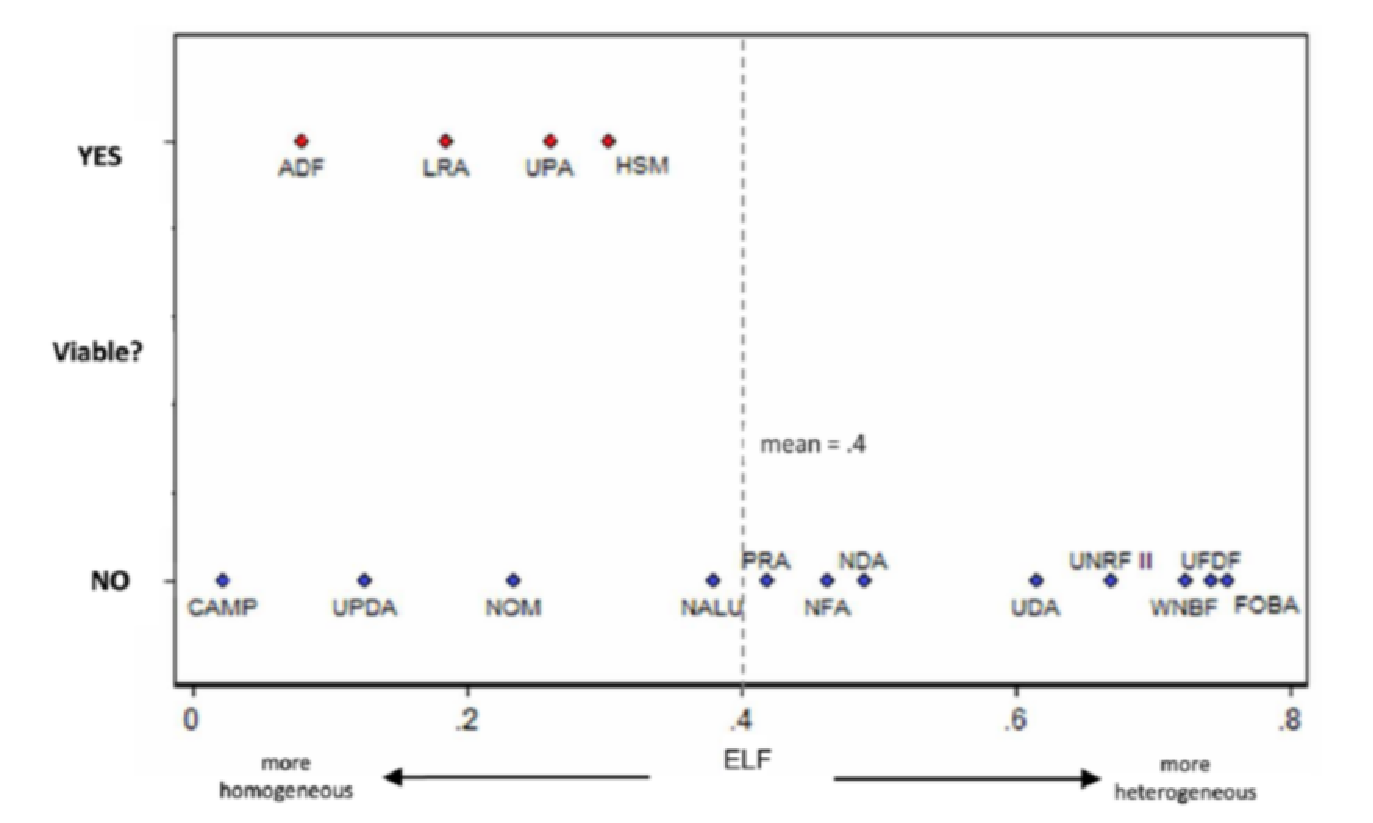
\includepdf[pages={1}]{Lewis_rebels.pdf}

\begin{frame}
\frametitle{Heterogeneity Tests}
\begin{itemize}
\item Sometimes the implications of theory are very precise
\item Treatment is likely to have affected subgroups to different degrees
\item We can use heterogeneity tests to disaggregate the effect to each subgroup and compare
\end{itemize}
\end{frame}

\begin{frame}
\frametitle{Heterogeneity Tests}
\begin{itemize}
\item For example, Ferraz and Finan (2008) ask how random audits affect corruption rates
\item They find that audits significantly reduce corruption
\item But their theory is that this is produced by 'electoral accountability' 
\item They provide evidence for this specific theory by:
\begin{itemize}
\item Subsetting the data to only those municipalities with local radio stations which broadcast the findings of corruption and showing the effect is much \textit{stronger}
\item Subsetting the data to only those municipalities with mayors in their first-term and face re-election incentives, showing corruption is lower
\end{itemize}
\item What other theory would be consistent with \textit{all} of these findings?
\end{itemize}
\end{frame}

\begin{frame}
\frametitle{Placebo tests}
\begin{itemize}
\item Our theory has very precise implications, and we normally test the 'positive' version
\item But we can also test the 'non-predictions' of our theory, when there should \textit{not} be an effect
\item If we found an effect where there should \textit{not} be one, we might think something is weird in our data/methodology and have less confidence in our main result
\end{itemize}
\end{frame}

\begin{frame}
\frametitle{Placebo tests}
\begin{itemize}
\item For example, with a regression discontinuity on close elections we expect a 'jump' effect when elections are tied (winning margin=0)
\item We expect there \textit{not} to be a 'jump' effect when winning margin=10\%
\begin{itemize}
\item In fact, RDDs assume continuity away from the threshold, so we need there to be no jump
\end{itemize}
\item So we can apply our regression discontinuity again and see what the effect is at winning margin=10\%
\item If we still find an effect, there might be something wrong with our data/method
\end{itemize}
\end{frame}

\begin{frame}
\frametitle{Placebo tests}
\begin{itemize}
\item The same with difference-in-differences
\item If we were estimating the effect of a treatment that applied to some units on 5th August 2012, we expect no effect on 3rd July 2009
\begin{itemize}
\item Or on 4th August 2012
\item Or on 6th August 2012
\end{itemize}
\item The more tightly the data are consistent \textit{only} with your theory, then the more credible your theory is
\end{itemize}
\end{frame}

\begin{frame}
\frametitle{Placebo tests}
\begin{itemize}
\item Placebo tests also work for small-N studies (Glynn and Ichino 2012)
\item We want to assess the effect of presidentialism on reducing party cohesion
\item A good comparison is between the USA (presidential) and Canada (parliamentary)
\item But we also gain confidence if we can show that other similar parliamentary systems have cohesive parties (Britain, Australia, etc.)
\end{itemize}
\end{frame}

\begin{frame}
\frametitle{Mechanisms}
\begin{itemize}
\item Often we talk as though we are testing 'treatments'
\begin{itemize}
\item But that leaves an empty black box between treatment and outcome
\end{itemize}
\item Really we want to test \textbf{theories}, which include a clear logical connection between the treatment and the outcome
\item To show that a specific theory is operating, we want to trace every step of the mechanism
\end{itemize}
\end{frame}

\begin{frame}
\frametitle{Mechanisms}
\begin{itemize}
\item For example, multiple studies show a clear treatment effect: high ethnic diversity reduces public goods provision
\begin{itemize}
\item But these studies had \textit{no theory}
\end{itemize}
\item Habyarimana et al (2007) asked "why?"
\begin{itemize}
\item Preferences
\item Technology
\item Strategy selection
\end{itemize}
\item They designed laboratory games to test exactly each mechanism
\item Eg. To test if there is an ethnic 'technology' that helps co-ethnics, they asked Ugandans to find a specific person in a neighbourhood, and paid them a reward if they did
\begin{itemize}
\item Co-ethnics found their target 43\% of the time, non-co-ethnics only 28\% of the time
\end{itemize}
\end{itemize}
\end{frame}

\begin{frame}
\frametitle{Mechanisms}
\begin{itemize}
\item Process Tracing is one way of demonstrating which mechanism connected the treatment and the outcome 
\end{itemize}
\end{frame}

\begin{frame}
\frametitle{Mechanisms}
\begin{itemize}
\item Brady (2004) provides an example of process tracing to evaluate the plausibility of a difference-in-differences research design
\item Difference-in-differences analysis suggested media announcements that Al Gore won Florida in 2000 caused 10,000 Gore voters to stay at home, allowing Bush to win.
\item But:
\begin{itemize}
\item There were only 10 minutes until the polling stations closed
\item Only 20\% heard the announcements
\item Around half were Bush voters, who may also have stayed home
\item Voters still had a reason to vote for other offices
\end{itemize}
\item Brady estimates that at most 224 people did not vote due to the media announcements
\end{itemize}
\end{frame}

 
\end{document}
 % effects of causes vs. reverse
